\chapter{法文文档}

\begin{quote}
    那人说,你所赐给我,与我同居的女人,她把那树上的果子给我,我就吃了。
    
    \hfill《圣经·创世纪》3:12
\end{quote}

了解法文文档要遵循的规则总是好的。严格说来,这些规则并不是无法逃避的准则,而更像是一些使用上的规矩。为了让文档容易可读、避免读者被打断,\emph{建议遵循}这些规则。这些使用上的建议总体上可以让文档看起来更严肃,甚至更专业。有很多关于法文排版的作品,这里给出来自国家印刷局(imprimerie nationale)的汇编材料[7],以及伊夫·佩伊卢梭(Yves Peyrousseaux)的手册[13]。

本章包含一些总结了有关\LaTeX 为实现法文变音符号而使用的字体编码方法的信息,介绍了关于排版的一些规则和用于简化法文输入过程的包\textsf{babel}。本章的末尾介绍了文档类型\dm{letter},其是为信件和传真而设计的。

\section{带有变音符号的字母的问题}

在若干年前,\TeX 的构思阶段完成的时候,其使用的字体不包含带有变音符号的字符。每个字形以7个二进制位区分,这样一共有128个字符可被编码。由于这种方法起源于美国,这128个字符中显然不包括法文中使用的带有变音符号的字符。正因如此,在很长一段时间内,那些优秀的讲法语母语的\TeX 和\LaTeX 用户不得不以一种窘迫方式去录入带有难以输入的字符的法文文档(document en \verb+fran\c{c}ais+ avec des \verb+caract{\`e}res+ assez \verb+p{\'e}nibles+ \verb+{\`a}+ taper)\yz{
    即document en français avec des caractères assez pénibles à taper。原书此处以源代码的方式展示部分单词,以展现其烦琐程度。%原书依然错误渲染了上引号和下引号
}。

今天,这些不悦不再成为人们的糟糕记忆。1990年起,一种容纳了多种语言中带变音符号的字符的字体编码被采用,称为\emph{Cork encoding}或\emph{T1编码(codage T1)}。当然,这种\TeX 编码本身和目前的字符编码标准间存在一定的联系。一些\LaTeX 包就包含了从字符编码(如iso-latin1)到字体编码(如T1编码)的“翻译”操作。

\begin{exclamation}
    于20实际90年代末出现的标准是ISO8859,带有针对称为\emph{latin1}的欧洲语言的编码方案扩展。这也是今天最常用的编码方案。然而,近年来,通用的字符表格\emph{统一码(Unicode)}及其编码\dm{UTF-8}标准得到了大多数系统的良好支持。不幸的是,\LaTeX 引擎最初并没有考虑处理含以多个字节存储的带有变音符号的字符的文档的情况\jz{这正是\dm{UTF-8}面临的情况。}。因此,有多种新型引擎见于公众,如pdftex、xe\TeX 、lua\TeX ,但它们暂时都没有被社区承认为标准。因此,编译以\dm{UTF-8}编码的文件时,需要在这些引擎中自行选用。本书创作时,选用了编码ISO88559和引擎pdftex。
\end{exclamation}

\section{使用\LaTeX 以法文创作}

有两个\LaTeX 包可以将文档“法国化”:\textsf{french}和\textsf{babel}。我们凭借带有绝对偏见的理由选用了后者,使用以下方法激活了包\textsf{babel}:

\begin{dmd}
\verb|\usepackage[francais]{babel}|
\end{dmd}

这条指令出现在文前部分,它使得五个功能运转起来,具体如下。

\begin{description}
    \item[断字] \textsf{babel}在处理段落中的断字时,会考虑法文的使用习惯\jz{
        英文单词和法文单词需要依据不同的规则打断。
    },尤其是会特殊考虑带有变音符号的法文单词。
    \item[排版] 应用法文的排版规则,特别是在面对涉及引号和其他标点符号的情况时。
    \item[版式] 主要涉及为章节标题后的首段文字重新引入首行缩进\jz{在英文排版时不需引入。},为列表替换符号、调整空白等。
    \item[翻译] 将敏感词翻译为法文,如“章”(chapitre)、“目录”(table des matières)等。
    \item[宏] 包\textsf{babel}中提供了一组可用的宏,用于插入一些法文中日常使用的结构,如no、1er、2o、37°C等。
\end{description}

\section{包\textsf{babel}和排版}

与法文排版相关的“规则”集合远远超出了本章的框架。幸运的是,包\textsf{babel}从实践的角度,允许我们在不了解这些规则的情况下去使用它们。我们只需简单地遵守\LaTeX 文档的几条\emph{输入}规则,就能使编译结果遵循那些最常用的排版规则。举例来说,\textsf{babel}会自动在分号前插入一个无法打断的四分之一全空格\yz{全空格(cadratin)指当前字体下字符M的宽度。}。对于法文排版,这是十分常见的做法。

\begin{ii}
如果你不想自动插入此类空格,可以调用指令\verb|\NoAutoSpaceBeforeFDP|。这样一来,你就可以全权决定是否在标点符号前插入空格。
\end{ii}

\subsection{标点符号}

关于标点符号,需要你了解的规则可以总结为以下两点。

\begin{enumerate}
    \item \emph{双}标点——即; : ! ? « »——的前后都应该添加空格。
    \item \emph{单}标点——即. , ( )——的后面应当插入空格,而前面不需要\yz{此处显然是原书纰漏了,左圆括弧的空格应当加在括弧外,即前面。}。
\end{enumerate}

以遵循上述规则的方式输入文档,\textsf{babel}就可以在标点符号前后自动插入空格。对于这个话题,有个有趣的知识点——问号和句号前的空格会更窄一些:

\begin{codelist}[7.1]{
    fouilla\,! et\enspace\,fouilla !
}\begin{verbatim}
fouilla ! et \selectlanguage{english}
fouilla !\selectlanguage{french}
\end{verbatim}
\end{codelist}

\subsection{L-a, e dans l'a, t-i, t-i, a !}

我改编了塞尔日·甘斯堡(Serge Gainsbourg)的歌词作为本小节的标题\yz{
    原歌词为“Elaeudanla teïtéïa”,出自歌曲\emph{Elaeudanla téitéia}。该句歌词描述了拼读Lætitia一词时的发音,其中将æ读作“a, e dans l’a”,即拆读为“a”和“那a中的e”。Lætitia为人名。作者以更贴近Lætitia一词的形式重新拼写该发音作为本小节标题。
},来借此介绍法文中的两个“美丽”的合字:æ和œ。为了输入这两个合字,我们可以选择输入\verb|\ae|和\verb+\oe+(对于大写,则使用\verb|\AE|和\verb+\OE+):

\begin{codelist}[7.2]{
    拉蒂希娅(L\ae titia)去了圣心教堂(Sacré-C\oe ur)。
}\begin{verbatim}
拉蒂希娅(L\ae titia)去了圣心教堂(Sacré-C\oe ur)。
\end{verbatim}
\end{codelist}

如果你的键盘允许,也可以直接输入æ。作为参考,在Linux系统上使用组合键\ovalbox{Alt Gr}+\ovalbox{A}可以输入名副其实地得到这种“a中的e”。出于历史原因,“o中的e”不在范式iso-latin1中,我的键盘不支持直接输入合字æ。

\subsection{包\textsf{babel}中的工具}

在排版时,“是否被排正确”这个问题对于大量细枝末节的内容是很难界定的,例如我想到的以下这些词的缩写:先生、女士、第一、第二、第一,等等。幸运的是,包\textsf{babel}在一定程度上解决了我们的问题。

\begin{center}
    \begin{tabular}{|l|l|}
        \hline
        \verb|1\ier| & 1er\\
        \verb|3\ieme| & 3e\\
        \verb|37\degres{} C| & 37° C\\
        \verb|\primo, \secundo, \tertio, \quarto| & 1o , 2o , 3o , 4o\\
        \verb|\no 4| & no\,4\\
        \verb|\No 4| & No\,4\\
        \hline
    \end{tabular}
\end{center}

\subsubsection{首字下沉}

\lettrine[lines=2]{在}{一些}文档中,我们可以看到\emph{首字下沉(lettrine)}的效果,正如本段所示。包\textsf{lettrine}和贝尔纳·高乐(Bernard Gaulle)的包\textsf{french}定义了此类指令。在本书第II部分,我们会向你介绍一个生成此类指令的\LaTeX 源代码示例。%TODOx2

\subsubsection{摘目}

在法文文档中,我们通常将目录插在文档末尾,而将摘目(sommaire)——目录的摘要——插在文档开头。包\textsf{french}中提供了指令\verb|\sommaire|。正如其名,该指令可以生成文档的摘目。再一次地,我们会在本书第II部分向你介绍生成此类摘目的方法。

\subsection{工具推荐}

包\textsf{babel}的接下来这些推荐使用的功能没有详细说明。它们都是些你可以在排版书籍中可以找到的建议。

\begin{itemize}
    \item 如果你的键盘支持,法文的引号可以直接使用“«”和“»”输入;如果不支持,可以借助小于号和大于号输入:\dm{<<}和\dm{>>}。此外,还可以借助\verb|\og|和\verb|fg|输入:
    
    \begin{codelist}[7.3]{
        Qu’on devra dans ce cas saisir « ainsi ».
    }\begin{verbatim}
Qu’on devra dans ce cas saisir
\og ainsi\fg{}.
    \end{verbatim}
    \end{codelist}

    \item “英文化”的引号可以使用单引号和反引号生成:\verb|``|和\verb|''|。无论如何,直接使用“\verb|"|”作为引号都是不推荐的。
    
    \item 拉丁短语\emph{理论上(a priori)}应以意大利体输入。
    
    \item 有以下缩写规则\jz{
        其中,Monsieur不应缩写为“Mr.”——这是英文\emph{mister}的缩写。
    }:

    \begin{center}
        \begin{tabular}{|l|l|l|}
            \hline
            \emph{et cætera} & 缩写为\quad \verb|etc.| & etc.而不是“etc...” \\
            Monsieur & 缩写为\quad \verb|M.| & M. Machin \\
            Messieurs & 缩写为\quad \verb|MM.| & MM. Machin et Bidule\\
            Madame & 缩写为\quad \verb|M\up{me}| & Mme Machin\\
            Mademoiselle & 缩写为\quad \verb|M\up{lle}| & Mlle Machin\\
            kilomètre(s) & 缩写为\quad \verb|km| & 25 km(不加s)\\
            kilogramme(s) & 缩写为\quad \verb|kg| & 25 kg\\
            \hline
        \end{tabular}
    \end{center}

    \item 法文中,整数与小数间的分割符为\emph{逗号},而英文中为圆点。因此我们“应当”这样写:123,54。
    
    \item 每逢千位或千分位\yz{即从小数分割符向两侧每三位。},要插入四分之一全空格:
    \begin{codelist}[7.4]{
        12\,345\,678,234\,34
    }\begin{verbatim}
\nombre{12345678,23434}
    \end{verbatim}
    \end{codelist}

    \item 可以将专有名词写成小型大写字母的形式,比如John \textsc{Coltrane}。这里使用的方式是\linebreak\verb|\textsc{Coltrane}|,但包\textsf{babel}中包含了宏\verb|\bsc|,可以忽略大小写。也就是说,\verb|\bsc{COLTRANE}|、\linebreak\verb|\bsc{Coltrane}|和\verb|\bsc{coltrane}|都可以生成预期的结果。
    
    \item 首字母缩合词应采用大写,并且不加圆点,如RATP\yz{全称为Régie autonome des transports parisiens,即巴黎独立运输公司。}、SNCF\yz{全称为Société nationale des chemins de fer français,即法国国家铁路公司。}、ENISE\yz{即国立圣-埃蒂安工程师学院。}。如果首字母缩合词“可以直接读出来”,则也可以使用小写字母,如Assedic\yz{全称为Association pour l ’Emploi dans l’Industrie et le Commerce,即工商业就业协会。}、Inserm\yz{全称为Institut national de la santé et de la recherche médicale,即全国保健和医学研究所。}等。
\end{itemize}

\subsection{欧元符号}

欧元符号可以借助包\textsf{textcomp}中的指令\verb|\texteuro|生成。因此,我们可以得到€。如果使用非衬线字体,则有\textsf{€}。另一种输入方式是借助包\textsf{eurosym},支持如下指令。

\begin{itemize}
    \item \verb|\euro{}|:€。
    \item \verb|\euro{35}|:35€。
\end{itemize}

\subsection{说到大写……}

除了耳熟能详的应当或不应当使用大写的情况(句首应大写,括号内首字母不应大写,冒号后取决于具体内容,等等),关于大写(majuscule;对于印刷工人,会称作capitale),有以下三个要点。

首先,\textbf{大写字母也应带有变音符号}(我没生气,我在解释)。伊夫·佩伊卢梭的手册中有关于此的说法:大写字母的变音符号自16世纪以来就一直存在,但随着盎格鲁-撒克逊人带来的打字机和印刷排版技术而消失了。我们同样可以在各种优秀的排版图书中找到因没有添加变音符号而导致歧义的例子。

其次,\emph{对于标题},我们只将全句的首字母大写(与此相反,英文中会将每个单词的首字母大写)。最后,需要强调,大写字母如何使用是很微妙的,大写字母的使用与否会带来微妙的差别。这里展示了一些示例,可以让你领会这些“规则”:

\begin{itemize}
    \item maître de conférences(也就是不用大写);
    \item l’université Jean Monnet(université一词不大写);
    \item 当谈论作为独立实体的结构时,写成l’Université;
    \item le ministre de l’Intérieur;
    \item l’académie de Lyon;
    \item l’Assemblée nationale、le Sénat,因为它们是独立机构;
    \item les Espagnols(指人)、le français(指语言)。
\end{itemize}

我不反对雅克·安德烈(Jacques André)的观点:

\begin{quote}
    ……我们在活动报告中找到了这样一句典型的话:
    
    \begin{quote}
        Jean Transent, Maître de Conférence en Analyse de Données à l’Université de Nancy (Bien connue de la Communauté Scientifique Internationale) a donné, lors du séminaire de Biologie Informatique de Mardi 23 Juin, une conférence sur les Applications de l’Intelligence Artificielle à l’emploi de la Télévision Haute Dé- finition en Robotique Avancée.
    \end{quote}

    这句话中共有23个大写字母,但按理来说,应当只有3个,分别用于Jean、Transent和Nancy。是的,没错……
    
    \hfill 雅克·安德烈[2]
\end{quote}

我也不反对伊夫·佩伊卢梭的观点:

\begin{quote}
    用于体现尊严、权力、等级或职能的名头\textbf{是普通的称谓}:
    \begin{itemize}
        \item ……
        \item 总理事会主席(le président du conseil général),等等。\\\textsf{这是个普通的称谓,就像总理事会保安或总理事会保洁一样。}
    \end{itemize}

    \hfill 伊夫·佩伊卢梭[13]
\end{quote}

\section{信件和传真}

\LaTeX 的核心包含了用于写信的文档类型。然而,这个类型不够灵活,也没有很好地兼容\linebreak 法文\jz{
    1999年2月9日基于文档类型\dm{class} 1.2z版本的个人评价。
}。对于法文信件,我们建议你使用来自日内瓦天文台的德尼·梅吉翁(Denis Megévand)开发的文档类型\dm{lettre}。该类型和其文档可以在\wz{obsftp.unige.ch/pub/tex/macros/lettre}找到,也可以在发行版Debian Sarge中的包\dm{tetex-frogg}中找到。

\subsection{可用指令}

以下是我们在信件类型中可以定义的几个实体。

\begin{description}
    \item[寄件人地址] 使用指令\verb|\address|。
    \item[出发地] 使用\verb|\lieu|可以在页面右上方书写下我们的信件来自何地。
    \item[电话和传真] 分别使用指令\verb|\telephone|和\verb|\fax|指明。
    \item[签名] 使用指令\verb|\signature|。
    \item[信件主题] 使用指令\verb|\conc|(指concernant,即“关于”)。
    \item[附件] 使用指令\verb|\encl|(指英文的\emph{enclosed}) 。
\end{description}

\subsection{基于类型\dm{lettre}的文档}

图\ref{fig:7.1}展示了使用类型\dm{lettre}的\LaTeX 文档骨架。指令\verb|\opening|和\verb|\closing|是必需的,分别对应在信件首尾引入礼貌用语的对象。

\begin{figure}[tb]
    \rotatebox{90}{%
      \begin{minipage}{.5\linewidth}
        \begin{footnotesize}
          \VerbatimInput{texs/ossature.tex}
        \end{footnotesize}
      \end{minipage}%
    \setlength{\fboxsep}{-\fboxrule}%
    \quad
    \fbox{\begin{minipage}{.7\linewidth}
        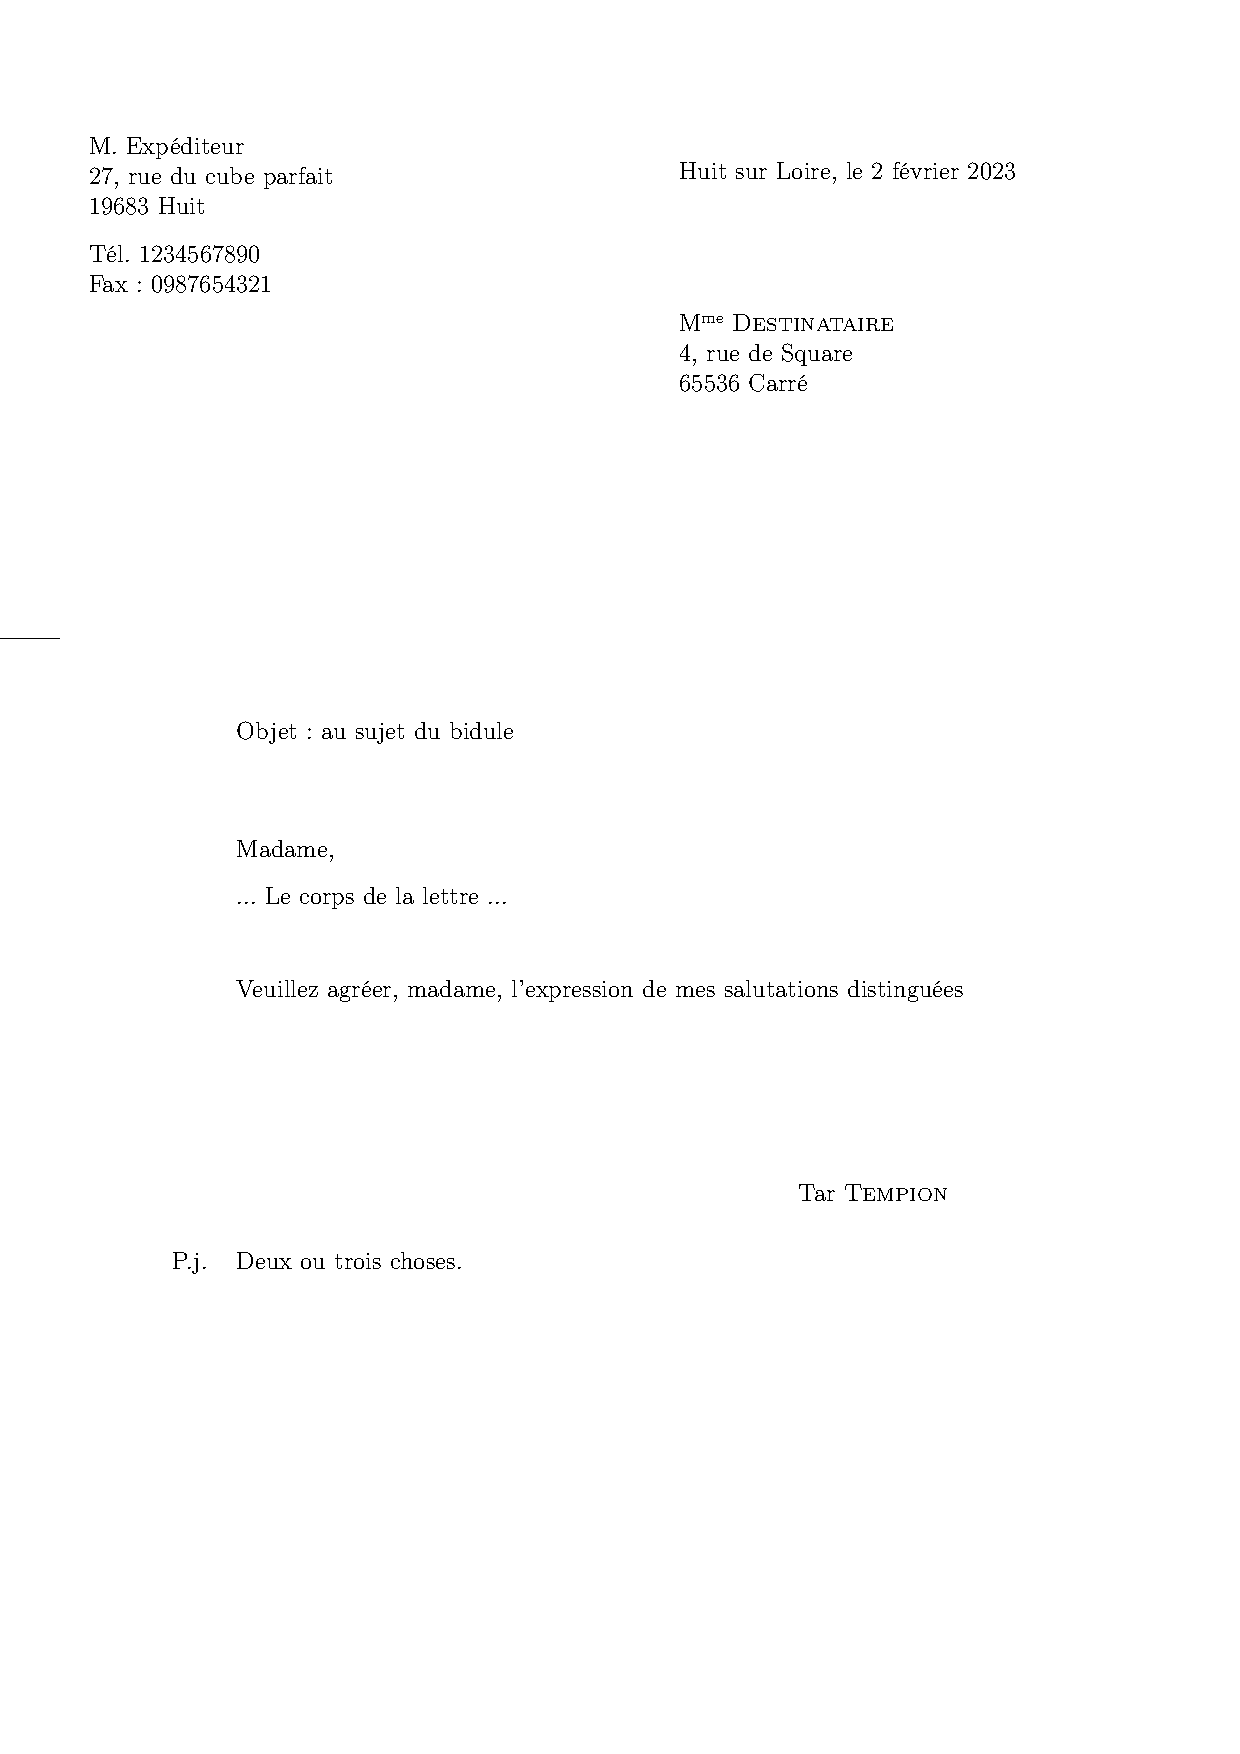
\includegraphics[width=\textwidth]{img/ossature}
      \end{minipage}}}
  \caption{基于类型\dm{lettre}的文档“骨架”}
  \label{fig:7.1}
  \end{figure}

\subsubsection{“协会”文件}

类型\dm{lettre}借助文件\dm{default.ins}交付。该文件默认定义了日内瓦天文台的地址。你使用的\LaTeX 系统管理员应当将该文件适配为你的组织。

我们可以定义自己的“协会”文件,并将其包含在信件中。但实际上,当我们想以私人名义寄信时,使用私人通信地址更符合逻辑。因此,我们可以定义名为\dm{moi.ins}的文件,并在其中包含相应信息,例如:

\begin{dmd}
\begin{verbatim}
\address{%
    M. Expéditeur\\
    27, rue du cube parfait\\
    19683 Huit}
\lieu{Huit sur Loire}
\telephone{1234567890}
\fax{0987654321}
\signature{Tar \textsc{Tempion}}
\end{verbatim}
\end{dmd}

此时,只需借助指令\verb|\institut|在文档的文前部分调用它。该指令会寻找带有扩展名\dm{.ins}的文件:

\begin{dmd}
\verb|\institut{moi}|
\end{dmd}

\subsection{传真}

信件类型中,同样包含用于传真的环境,它带有你所在组织的笺头。通用的原则和关键字与信件是相同的,只不过需要使用环境\dm{telefax}而不是环境\dm{letter}。

注意,这里我们仍然可以使用“机构”文件。毕竟,指令\verb|\addpages|可以用于需要在传真中附加已打印文档的情况。例如,你不得不向初始传真发送$n$页,就可以添加指令\verb|\addpages{|\codereplace{$n$}\dm{\}}。图\ref{fig:7.2}展示了创建传真需要的最小文档。



\begin{figure}[tb]
    \rotatebox{90}{%
      \begin{minipage}{.5\linewidth}
        \begin{footnotesize}
          \VerbatimInput{texs/ossature-fax.tex}
        \end{footnotesize}
      \end{minipage}%
    \setlength{\fboxsep}{-\fboxrule}%
    \quad
    \fbox{\begin{minipage}{.7\linewidth}
        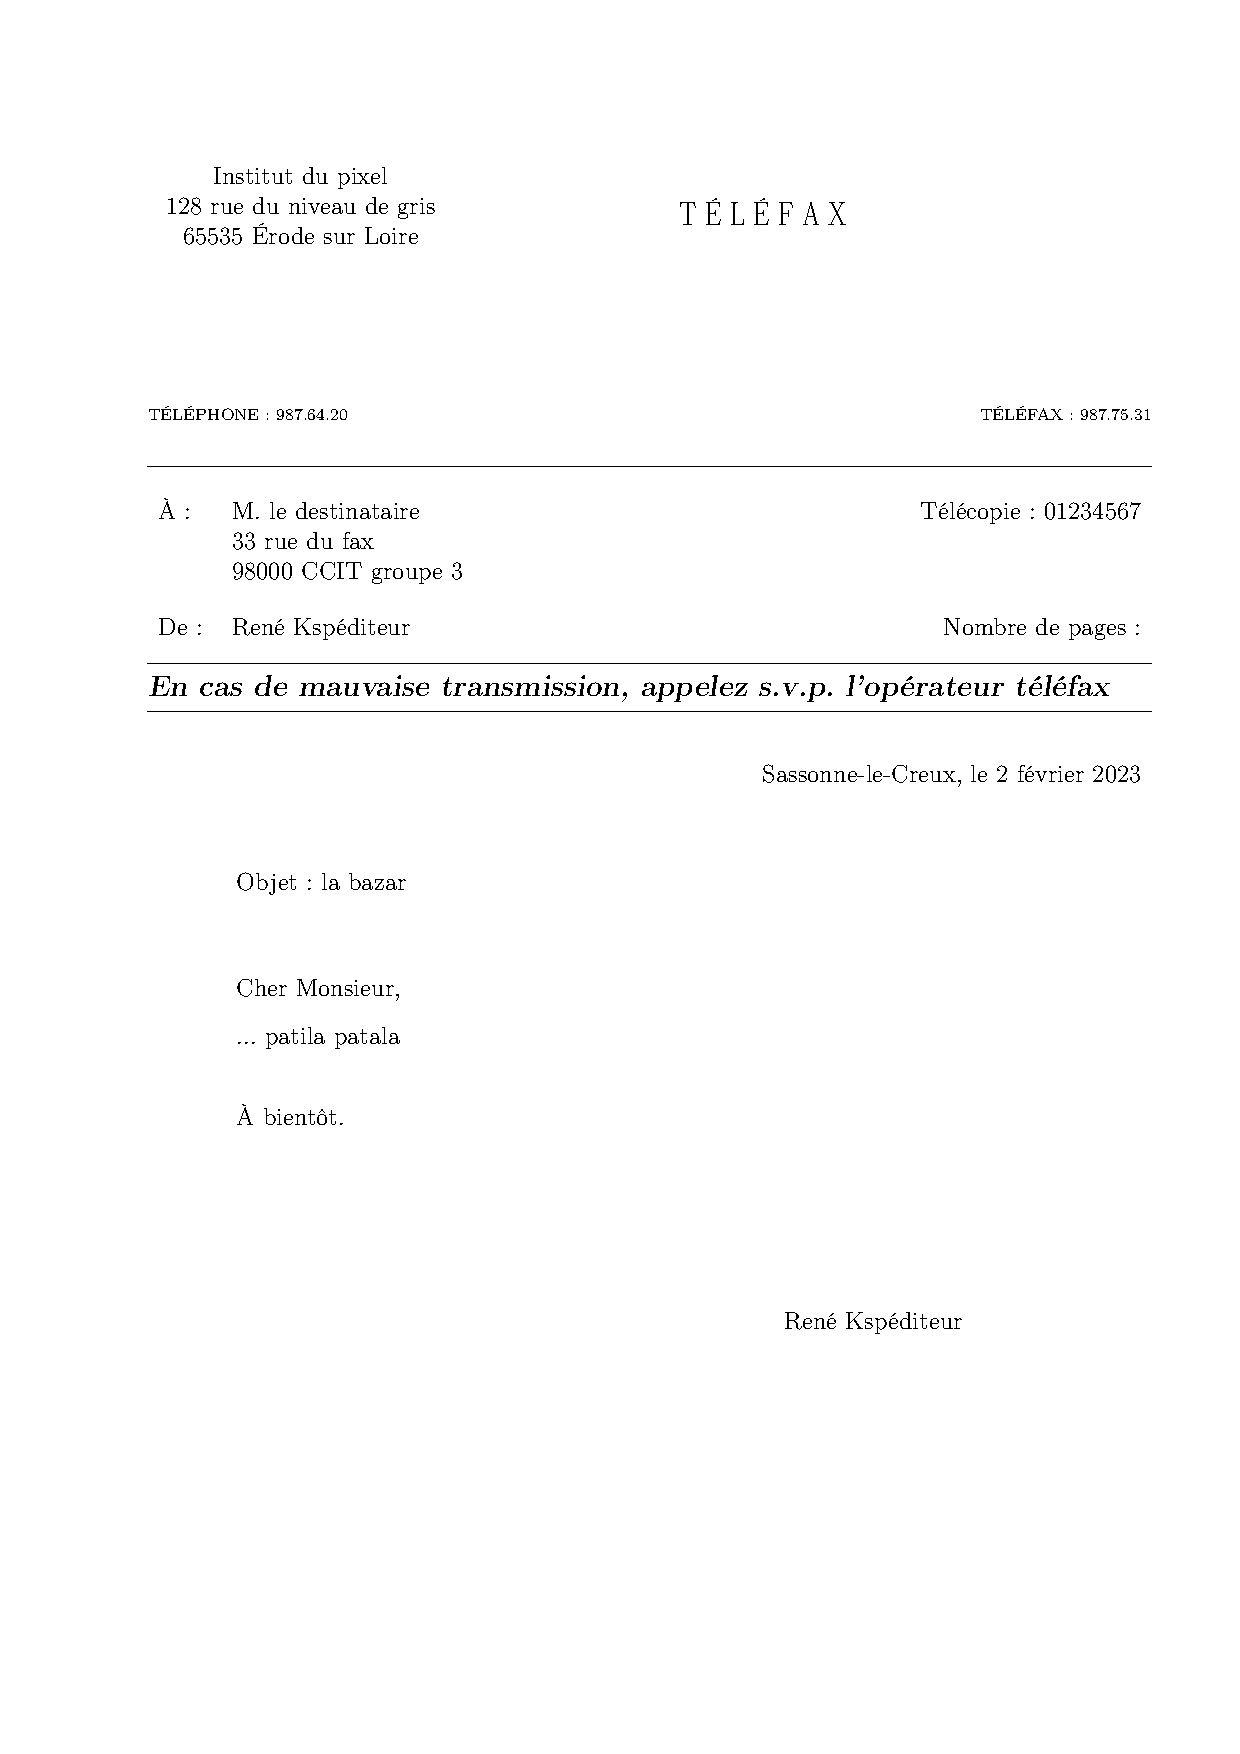
\includegraphics[width=\textwidth]{img/ossature-fax}
      \end{minipage}}}
  \caption{传真文档的“骨架”}
  \label{fig:7.2}
  \end{figure}